% ====================================================================
% COMPILACIÓN PRINCIPAL - TESIS DE GEOLOGÍA UCM 2026
% Estudiante: Francisco Sepúlveda Vergara
% Compañeros: Camila Orellana Garrido, Emilio Paineman, Ricardo Inostroza
% Asignatura: OPP125 - Herramientas Computacionales
% ====================================================================

\documentclass[12pt,letterpaper,oneside]{report}

% --- Paquetes obligatorios (Requisito pauta) ---
\usepackage[spanish,es-tabla]{babel} % Idioma español y cambia 'Cuadro' por 'Tabla'
\usepackage[utf8]{inputenc}          % Para poder escribir tildes y eñes directo
\usepackage{geometry}                % Para configurar los márgenes oficiales de tesis
\geometry{top=3cm, bottom=3cm, left=3.5cm, right=2.5cm}

\usepackage{graphicx} % Fundamental para cargar mapas y el logo de la UCM
\usepackage{amsmath}  % Para las fórmulas químicas de hidrólisis
\usepackage{fancyhdr} % Para personalizar la barra superior de las páginas
\usepackage{natbib}   % Para gestionar la bibliografía con BibTeX

% --- Configuración del encabezado ---
\pagestyle{fancy}
\setlength{\headheight}{16pt} % Ajuste para que no tire advertencia de tamaño
\fancyhf{}
\fancyhead[R]{\thepage}
\fancyhead[L]{\slshape \leftmark}
\renewcommand{\headrulewidth}{0.4pt}

\usepackage{xcolor}
\usepackage{chngcntr}
\counterwithout{figure}{chapter} % Quita la dependencia del capítulo (se convierte en Figura 1, 2, 3...)

% --- Comentarios y ediciones del revisor ---
\newcommand{\naty}[1]{\textcolor{blue}{#1}}
\newcommand{\coment}[1]{\textcolor{red}{\textbf{[Comentario: #1]}}}

% ====================================================================
% APERTURA DEL DOCUMENTO
% ====================================================================
\begin{document}

% --- 1. PORTADA OFICIAL ---
\begin{titlepage}
    \centering
    
    % Aquí va el logo institucional (el archivo debe estar subido en la carpeta imagenes)
    
\includegraphics[width=1.1\textwidth]{imagenes/logo_ucm.png}\\[1.2cm] 
    
    {\bfseries\Large UNIVERSIDAD CATÓLICA DEL MAULE}\\[1cm]
    {\small FACULTAD DE CIENCIAS BÁSICAS}\\[0.2cm]
    {\small ESCUELA DE GEOLOGÍA}\\[2.5cm]
    
    {\Large\bfseries De la roca a la costa: fuentes geológicas potenciales de hierro y rutas de transporte en la Región del Maule, Chile}\\[2.5cm] 

    {\large Optativo de Investigacion Aplicada GEO225}\\[2.5cm]
    
    \begin{flushright}
        \textbf{Autor/a:} Francisco Sepúlveda Vergara\\[0.2cm]
        \textbf{Profesor Guía:} Dr. Natalia Opazo\\[0.2cm]
    \end{flushright}
    
    \vfill
    {\large Talca, 2026}
\end{titlepage}

% --- 2. PÁGINAS PRELIMINARES E ÍNDICES ---
\clearpage
\pagenumbering{roman} % Números romanos (i, ii, iii) para las primeras hojas

% ====================================================================
% SECCIÓN MODULAR: PÁGINAS PRELIMINARES DE LA TESIS
% Requisito de la pauta: Incluir dedicatoria, agradecimientos y abstracts
% ====================================================================

% --- Nota: Dejar la dedicatoria lista al final, por ahora va este borrador ---
\thispagestyle{empty}
\vspace*{5cm}
\begin{flushright}
    \textit{Dedicado a mi familia, amigos y a quienes apoyaron y se sientan parte, \\ también a los muchos que faltarán.}
\end{flushright}

\newpage

% --- Sección de Agradecimientos ---
\section*{Agradecimientos}
% Nota: Texto de ejemplo.
Agradezco a la Universidad Católica del Maule y a la Facultad de Ciencias Básicas 

\newpage

% --- Resumen del proyecto ---
\section*{Resumen}
El hierro (Fe) constituye un micronutriente esencial para diversos procesos biogeoquímicos marinos y puede influir sobre la productividad primaria y la eficiencia de la bomba biológica de carbono. En este contexto, el aporte de hierro desde fuentes continentales y su posterior movilización y transporte constituyen procesos relevantes para comprender la disponibilidad de este elemento en los sistemas acuáticos. Sin embargo, la identificación de una fuente potencial de hierro requiere considerar no solo su composición, sino también las características del material y las condiciones ambientales que pueden favorecer su movilización y transporte.

El presente trabajo tiene como objetivo evaluar el potencial de fuentes geológicas de hierro y sus posibles rutas de transporte en un área de estudio acotada de la Región del Maule, mediante la integración de antecedentes geológicos, geoquímicos, geomorfológicos, topográficos, hidrológicos y climáticos. Para ello, se propone desarrollar una base de datos espacial que permita caracterizar potenciales fuentes de hierro y analizar su conectividad mediante posibles rutas de transporte fluvial y atmosférico, considerando diferentes condiciones de movilización y las incertidumbres asociadas a la información disponible.

Durante esta etapa se realiza una revisión bibliográfica orientada a establecer el marco conceptual del estudio, abordando la bomba de tejidos blandos, la función del hierro en la biogeoquímica oceánica, las características de las partículas minerales y los procesos asociados a su movilización y transporte. Asimismo, se contempla la recopilación y organización de información geoespacial y temática necesaria para la construcción de la base de datos y el posterior análisis espacial. La metodología propuesta permitirá desarrollar una aproximación exploratoria al sistema fuente--transporte--receptor, orientada a identificar zonas con condiciones potencialmente favorables para constituir fuentes de hierro y sus posibles conexiones con sistemas fluviales y ambientes costeros.

\vspace{1.5cm} % Para separar ordenadamente ambos textos

% --- Abstract en inglés (Cambiando el idioma con babel) ---
%\selectlanguage{english}
%\section*{Abstract}
%Texto aqui.
\selectlanguage{spanish} % volver al español aquí para no romper el formato

\tableofcontents
\listoffigures
\listoftables

% --- 3. CUERPO DE LA TESIS (Modulares) ---
\clearpage
\pagenumbering{arabic} % Cambiamos a números normales (1, 2, 3...) para el desarrollo

% ====================================================================
% CAPÍTULO 1: INTRODUCCIÓN Y PLANTEAMIENTO GEOLÓGICO
% ====================================================================
\chapter{Introducción}
% Nota personal: 

El océano desempeña un papel fundamental en la regulación del ciclo global del carbono, participando en el intercambio de dióxido de carbono ($CO_2$) entre la atmósfera y los sistemas marinos \citep{HainSigman2014}. Dentro de este sistema, una de las vías mediante las cuales el carbono puede ser transferido desde las aguas superficiales hacia el océano profundo corresponde a la denominada bomba biológica \citep{HainSigman2014}. Este proceso se encuentra asociado principalmente a la producción de materia orgánica mediante la actividad fotosintética de organismos marinos y a la posterior exportación de una fracción de dicha materia hacia mayores profundidades, donde parte del carbono puede permanecer aislado de la atmósfera durante períodos prolongados \citep{HainSigman2014}.

La eficiencia de la bomba biológica está condicionada por diversos factores físicos, químicos y biológicos, entre ellos la disponibilidad de luz, la temperatura, la circulación y estratificación de la columna de agua, la disponibilidad de nutrientes y la actividad de los organismos que consumen y remineralizan la materia orgánica. Entre los nutrientes esenciales para la productividad primaria destaca el hierro (Fe), un micronutriente cuya disponibilidad puede limitar el crecimiento del fitoplancton incluso en regiones oceánicas donde existen concentraciones relativamente elevadas de macronutrientes, como nitrógeno y fósforo \citep{Tagliabue2017}. El hierro participa en procesos metabólicos fundamentales, como el transporte de electrones durante la fotosíntesis y la respiración celular, y forma parte de proteínas y enzimas involucradas en la utilización de energía y nutrientes. Por ello, su disponibilidad puede influir en la productividad primaria y en la cantidad de materia orgánica producida, aunque la proporción que finalmente alcanza el océano profundo también depende de los procesos de hundimiento, consumo y remineralización \citep{Tagliabue2017}.

El hierro que ingresa a los sistemas oceánicos puede presentar diversos orígenes y encontrarse asociado a diferentes procesos de movilización y transporte. Si bien el aporte de partículas minerales mediante transporte atmosférico ha sido ampliamente estudiado, investigaciones recientes han destacado la importancia de considerar la diversidad de fuentes, caracteristicas mineralogicas y procesos que controlan la disponibilidad del hierro. factores como la composicion mineralogica, el tamaño de las particulas, el grado de alteracion y las transformaciones experimentadas durante el transporte pueden influir sobre la solubilidad y, por esto, sobre la fraccion de hierro potencialmente disponible para los organismos marinos \cite{Zan2025}. De esta manera, la identificacion de una fuente potencial de hierro requiere considerar no solamente su contenido total de este elemento, si no tambien las condiciones que pueden favorecer su movilizacion y posterior transporte.

En este contexto, las características geológicas y ambientales de las zonas continentales pueden constituir un componente relevante para comprender el origen y las posibles rutas de transporte de partículas ricas en hierro hacia sistemas acuáticos. La movilización de material particulado puede estar condicionada por factores como la disponibilidad de sedimentos, las condiciones del suelo y la cobertura vegetal, mientras que su transporte puede depender de variables atmosféricas, topográficas e hidrológicas \citep{Zan2025}. Por lo tanto, la identificación de potenciales fuentes de hierro requiere integrar información proveniente de distintas disciplinas, considerando tanto las características del material como las condiciones ambientales que podrían favorecer su movilización y transporte.

A partir de lo anterior, el presente trabajo busca evaluar el potencial de determinadas fuentes geológicas de hierro y sus posibles rutas de transporte dentro de un área de estudio acotada de la Región del Maule. Para ello, se plantea la integración de antecedentes geológicos, geoquímicos, geomorfológicos, topográficos, hidrológicos y climáticos mediante herramientas de análisis espacial y computacional. El enfoque considera una perspectiva de fuente--transporte--receptor, orientada a identificar espacialmente zonas que presenten condiciones potencialmente favorables para actuar como fuentes de hierro y analizar su posible conectividad con sistemas fluviales y ambientes costeros.

La integración de estas variables permitirá desarrollar una primera aproximación espacial a la distribución de potenciales fuentes de hierro y a los procesos que podrían favorecer su movilización y transporte. Debido a la naturaleza exploratoria del estudio, los resultados serán interpretados en términos de potencialidad y escenarios de movilización, considerando las incertidumbres asociadas a la disponibilidad y calidad de los datos utilizados.

%\section{Planteamiento del Problema}
% Nota: Aquí se explico la contradicción geológica que da origen a la tesis.
%El problema geológico radica en caracterizar el mecanismo... \coment{Esta sección no es necesaria, el planteamiento del problema ya se encuentra en la introducción.}

\section{Hipótesis de Trabajo}%Con formato de hipotesis tal cual H0: hipotesis nula.

\textbf{H$_0$: Hipótesis nula.} La integración de antecedentes geológicos, mineralógicos, geoquímicos, geomorfológicos, topográficos, hidrológicos y climáticos de la Región del Maule no permite distinguir sectores con condiciones relativamente más favorables para constituir fuentes potenciales de hierro ni establecer diferencias espaciales fundamentadas en su posible conectividad con ambientes costeros.

\medskip

\textbf{H$_1$: Hipótesis alternativa.} La integración de antecedentes geológicos, mineralógicos, geoquímicos, geomorfológicos, topográficos, hidrológicos y climáticos de la Región del Maule permite distinguir sectores con condiciones relativamente más favorables para constituir fuentes potenciales de hierro y reconocer posibles conexiones de transporte hacia ambientes costeros.

\section{Objetivos de la Investigación}

\subsection{Objetivo General}
Evaluar exploratoriamente el potencial de fuentes geológicas de hierro y sus posibles rutas de movilización y transporte hacia ambientes costeros de la Región del Maule, mediante la integración de antecedentes geológicos, geoquímicos, geomorfológicos, topográficos, hidrológicos y climáticos.

\subsection{Objetivos Específicos}
% Nota para el formato: Usar la lista con viñetas para ordenar las metas del proyecto.
\begin{itemize}
    \item Caracterizar las principales unidades geológicas y materiales superficiales del área de estudio con potencial para actuar como fuentes de hierro, considerando antecedentes litológicos, mineralógicos, geoquímicos, granulométricos y de alteración.
    \item Construir una base de datos geoespacial que integre antecedentes geológicos, geoquímicos, topográficos, hidrológicos y climáticos relevantes para la identificación y evaluación de fuentes potenciales de hierro.
    \item Analizar la conectividad potencial entre las fuentes identificadas y los posibles receptores mediante rutas de transporte fluvial y atmosférico, utilizando herramientas SIG y computacionales.
\end{itemize}
% ====================================================================
% CAPÍTULO 2: MARCO TEÓRICO
% ====================================================================
\chapter{Marco Teórico}
% Nota de avance: Revisión bibliográfica
%{2.1. Ciclo del carbono y bomba biológica de carbono
%Explicar el concepto, la exportación de materia orgánica y la conexión general con el ciclo del carbono. Evitar extenderse en procesos que no se medirán en el estudio.
%2.2. Hierro y productividad oceánica
%Integrar productividad primaria, funciones biológicas del Fe, limitación por nutrientes y fertilización con hierro. Explicar brevemente las regiones HNLC como ejemplo relevante, no como subsección independiente.
%2.3. Fuentes geológicas de hierro: litología y mineralogía
%Nueva sección prioritaria: minerales portadores de Fe, rocas y sedimentos potencialmente relevantes, composición geoquímica y diferencia entre contenido total y fracción potencialmente movilizable.
%2.4. Meteorización y generación de materiales superficiales
%Procesos de alteración física y química, formación de suelos y sedimentos, liberación potencial de Fe y controles geológicos y geomorfológicos.
%2.5. Movilización y transporte de materiales hacia la costa
%Diferenciar el transporte fluvial del atmosférico. Explicar qué datos permitirían evaluar cada vía y cuáles son las limitaciones para inferir conectividad.
%2.4 y 2.5 pueden ser complementarios por lo que se evaluo el orden o combinacion de estos puntos
%2.6. Enfoque fuente–transporte–receptor y aplicación regional}

\section{Ciclo global del carbono y bomba biológica de carbono}

El ciclo global del carbono comprende los procesos mediante los cuales este elemento se intercambia y almacena entre los principales reservorios del sistema Tierra, incluidos la atmósfera, los océanos, la biosfera y la litosfera. En el ambiente marino, el intercambio de dióxido de carbono (CO$_2$) entre la atmósfera y el océano, junto con los procesos biológicos, químicos y físicos que redistribuyen el carbono en la columna de agua, desempeña un papel fundamental en la regulación del clima a escala global. La magnitud de estos intercambios depende de factores como la circulación oceánica, la temperatura, la química del agua de mar y la actividad de los organismos marinos \citep{HainSigman2014}.

% --- Inserción de Figura  ---
\begin{figure}[h]
\centering
% Nota: Añadimos otra imagen en la carpeta de imagenes para esta parte
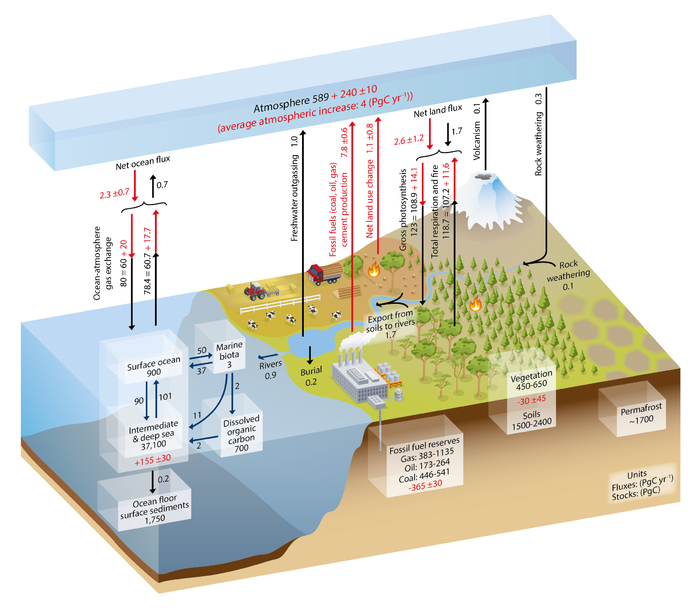
\includegraphics[width=0.8\textwidth]{imagenes/Ciclo_del_carbono.jpg}
\caption{Esquema simplificado del ciclo global del carbono. Las cantidades en los reservorios están en PgC y los flujos anuales en PgC año\textsuperscript{-1}. Los números y flechas negras indican los valores previos a la Era Industrial (~1750), mientras que los rojos representan los flujos antropogénicos (2000–2009) y los cambios acumulados (1750–2011). Tomado de \cite{Ciais2013}.}
\label{fig:ciclo_carbono}
\end{figure}

Uno de los mecanismos que interviene en la transferencia de carbono desde las aguas superficiales hacia el océano interior es la bomba biológica de carbono. Este proceso comienza cuando los organismos fotosintéticos, principalmente el fitoplancton, utilizan la energía solar para incorporar carbono inorgánico disuelto y producir materia orgánica. Una fracción de esta materia orgánica es consumida, transformada y remineralizada en las aguas superficiales; otra parte se exporta hacia mayores profundidades, principalmente mediante el hundimiento de partículas orgánicas, aunque también intervienen mecanismos de transporte asociados a organismos y a la circulación del agua. Cuando la materia orgánica se remineraliza en profundidad, el carbono vuelve a formas inorgánicas disueltas, lo que contribuye a mantener una distribución vertical del carbono diferente de la que existiría en ausencia de estos procesos \citep{HainSigman2014}.

La eficiencia de la bomba biológica no depende exclusivamente de la cantidad de carbono fijado durante la fotosíntesis. También está condicionada por la proporción de materia orgánica que logra escapar de la remineralización en las capas superficiales y alcanzar mayores profundidades. Por esta razón, la productividad primaria, la composición de las comunidades biológicas, la agregación y el hundimiento de partículas, y las tasas de consumo y descomposición de la materia orgánica son factores relevantes para comprender la magnitud de la exportación de carbono. En consecuencia, un aumento de la productividad superficial no implica necesariamente un incremento proporcional del almacenamiento de carbono en el océano profundo \citep{HainSigman2014,Tagliabue2017}.

La disponibilidad de nutrientes constituye otro factor importante para el funcionamiento de la bomba biológica. Elementos como el nitrógeno, el fósforo y el hierro intervienen en el crecimiento y el metabolismo del fitoplancton, aunque sus funciones y concentraciones requeridas son diferentes. Mientras que el nitrógeno y el fósforo son macronutrientes necesarios en cantidades relativamente elevadas, el hierro es un micronutriente requerido en cantidades menores, pero esencial para diversos procesos celulares. Su escasez puede restringir la productividad primaria en determinadas regiones oceánicas y, por lo tanto, influir en la cantidad de materia orgánica disponible para su posterior exportación \citep{Tagliabue2017}.

La relación entre la disponibilidad de nutrientes, la productividad biológica y el almacenamiento de carbono ha sido especialmente relevante en estudios sobre la variabilidad climática del pasado. Durante los periodos glaciales se produjeron cambios en las emisiones de polvo mineral, en su transporte atmosférico y en su deposición sobre el océano. Estos cambios pudieron modificar el suministro de hierro y otros elementos a determinadas regiones marinas, con posibles efectos sobre la productividad y la bomba biológica de carbono. Sin embargo, la magnitud de dicha respuesta dependió de las características de las partículas depositadas, de la disponibilidad efectiva de sus nutrientes y de las condiciones oceanográficas y biológicas existentes \citep{Lambert2021,Zan2025}.

En este contexto, estudiar las fuentes potenciales de hierro y los procesos que controlan su movilización permite abordar una parte de las conexiones entre los sistemas terrestres y marinos. Desde una perspectiva geológica, este análisis requiere considerar no solo la presencia de minerales portadores de hierro en las rocas y los sedimentos, sino también los procesos de meteorización, erosión y transporte que podrían favorecer su incorporación a sistemas fluviales o atmosféricos. Esta aproximación permite establecer una base conceptual para investigar posibles aportes continentales de hierro sin asumir, de antemano, que estos se traducen necesariamente en una fertilización efectiva del océano.

\section{Hierro y productividad oceánica}

El hierro (Fe) es un elemento esencial para el funcionamiento de los organismos marinos fotosintéticos. Participa en proteínas y enzimas involucradas en el transporte de electrones, la fotosíntesis, la respiración celular y otros procesos metabólicos relacionados con el aprovechamiento de energía y la asimilación de nutrientes. Aunque su requerimiento biológico es relativamente bajo en comparación con el de los macronutrientes, su disponibilidad puede limitar el crecimiento del fitoplancton en determinadas regiones del océano \citep{Tagliabue2017}.

Esta limitación se observa, entre otros ambientes, en algunas regiones oceánicas conocidas como zonas de altas concentraciones de nutrientes y baja clorofila (HNLC, por sus siglas en inglés). En ellas, las concentraciones de macronutrientes pueden permanecer relativamente elevadas, mientras que la productividad fitoplanctónica se encuentra restringida, en parte, por la escasez de hierro disponible. Este comportamiento demuestra que la presencia de nutrientes en el agua no garantiza por sí sola una respuesta biológica elevada: también es necesario considerar qué elementos limitan el crecimiento y en qué formas químicas se encuentran disponibles \citep{Tagliabue2017}.

El hierro ingresa al océano mediante diversas vías, entre ellas la deposición atmosférica de polvo mineral y cenizas, los aportes fluviales, los intercambios con los sedimentos marinos y otros procesos asociados a la circulación y a la interacción entre el agua y los materiales geológicos. La importancia relativa de cada vía varía según la región y las condiciones ambientales. En el caso del polvo atmosférico, las partículas pueden recorrer distancias considerables desde sus áreas de origen antes de depositarse sobre la superficie oceánica. En el caso del transporte continental, los materiales erosionados pueden ser movilizados por escorrentía y sistemas fluviales, aunque su composición y destino dependen de las condiciones geológicas, geomorfológicas e hidrológicas de cada cuenca \citep{Tagliabue2017,Zan2025}.

Sin embargo, el contenido total de hierro de un material no equivale a la cantidad que puede incorporarse al agua de mar en formas aprovechables por los organismos. El hierro presente en partículas minerales puede encontrarse alojado en distintas fases y minerales, con diferencias importantes en su estabilidad y comportamiento químico. Por consiguiente, la disolución, la transformación de las partículas y las reacciones que ocurren durante el transporte y después de la deposición condicionan la fracción de hierro que puede pasar a la fase disuelta y permanecer disponible para los organismos marinos \citep{Tagliabue2017,Zan2025}.

En el polvo mineral, estas diferencias dependen, entre otros factores, de la mineralogía, la composición geoquímica, el tamaño de las partículas y el grado de alteración del material de origen. También pueden influir los procesos químicos experimentados durante el transporte atmosférico y las condiciones del medio receptor. Por esta razón, dos fuentes con concentraciones totales de hierro similares pueden presentar comportamientos diferentes en términos de solubilidad y potencial de suministro de hierro biológicamente disponible. La evaluación de una fuente potencial debe distinguir, por tanto, entre la abundancia de hierro, su susceptibilidad a ser movilizado y su posible disponibilidad biogeoquímica \citep{Zan2025}.

La relación entre el suministro de hierro y la bomba biológica de carbono debe interpretarse con la misma precaución. En condiciones donde el hierro limita el crecimiento del fitoplancton, un aporte adicional de hierro biodisponible puede favorecer el aumento de la productividad primaria. No obstante, la respuesta depende de la disponibilidad simultánea de otros nutrientes, de las condiciones físicas y químicas del agua, de la comunidad biológica y de los procesos que determinan el destino de la materia orgánica producida. En consecuencia, un mayor aporte de hierro no implica automáticamente un aumento equivalente de la exportación de carbono ni permite cuantificar, sin información adicional, un efecto sobre el CO$_2$ atmosférico \citep{Tagliabue2017,Lambert2021}.

Para la presente investigación, estos antecedentes permiten establecer una distinción fundamental entre una fuente geológica de hierro y una fuente capaz de contribuir efectivamente al suministro de hierro al ambiente marino. La primera puede reconocerse por la presencia de minerales portadores de Fe y por sus características litológicas y geoquímicas. La segunda requiere, además, evaluar si existen procesos que permitan la meteorización o fragmentación del material, su movilización y transporte, su conexión con un sistema receptor y, finalmente, condiciones que favorezcan la liberación del hierro. Esta distinción orienta el análisis de las fuentes potenciales de la Región del Maule y evita equiparar la presencia de mineralización con un aporte demostrado al océano.

\section{Fuentes geológicas de hierro: litología y mineralogía}

La identificación de fuentes geológicas potenciales de hierro requiere considerar la composición de las rocas y los sedimentos, los minerales que contienen este elemento y los procesos geológicos que controlan su distribución. El hierro se encuentra en una amplia variedad de materiales naturales, tanto en minerales primarios que forman parte de las rocas ígneas y metamórficas como en minerales secundarios generados durante la meteorización y la formación de suelos. Su concentración y asociación mineralógica varían según el origen del material, las condiciones de formación y los procesos de alteración que haya experimentado.

Desde el punto de vista mineralógico, el hierro puede formar parte de óxidos, hidróxidos, sulfuros, silicatos y otras fases minerales. Entre los minerales relevantes se encuentra la magnetita (Fe$_3$O$_4$), un óxido de hierro que puede presentarse como mineral accesorio en distintas rocas o concentrarse en cuerpos de mineralización. También existen otros minerales portadores de hierro, como la hematita (Fe$_2$O$_3$), minerales del grupo de los sulfuros y silicatos ferromagnesianos. La presencia de estas fases no implica que todas tengan el mismo comportamiento durante la meteorización ni que liberen hierro con la misma facilidad. Por ello, la identificación mineralógica debe complementarse, cuando la información lo permita, con antecedentes sobre la composición geoquímica, el estado de alteración y las características físicas del material.

La litología constituye un criterio inicial para reconocer materiales que podrían actuar como fuentes de hierro. Las rocas volcánicas, por ejemplo, pueden contener minerales ferromagnesianos y óxidos de hierro cuya abundancia depende de su composición y evolución magmática. Asimismo, ciertos sistemas magmático-hidrotermales pueden generar mineralizaciones en las que los óxidos de hierro se concentran en vetas, brechas o cuerpos irregulares. Por otra parte, los sedimentos derivados de la erosión de distintas unidades geológicas pueden incorporar fragmentos de minerales portadores de hierro y redistribuirlos dentro de las cuencas. En consecuencia, la evaluación de fuentes potenciales requiere examinar tanto las unidades rocosas como los materiales superficiales derivados de ellas.

Un ejemplo regional de mineralización de hierro corresponde a las denominadas Vetas del Maule, ubicadas en los remanentes del volcán La Zorra, dentro del Complejo Volcánico Laguna del Maule. \cite{Cofre2022} describe una mineralización de tipo óxido de hierro-apatito (IOA, por sus siglas en inglés), alojada en rocas andesíticas y caracterizada por la presencia de cuerpos de magnetita masiva, vetas de piroxeno-actinolita-magnetita, brechas hidrotermales con matriz de magnetita, magnetita diseminada y vetas de piroxeno-actinolita con cantidades variables de magnetita. El estudio integra observaciones de terreno, caracterización petrográfica y análisis mediante microsonda electrónica para examinar las características mineralógicas y geoquímicas de esta mineralización.

La investigación de \cite{Cofre2022} interpreta que la mineralización se formó durante una evolución desde condiciones magmático-hidrotermales hacia condiciones hidrotermales, con variaciones composicionales de la magnetita y temperaturas de formación estimadas aproximadamente entre 950 y 500 °C. Estos antecedentes permiten reconocer la existencia de materiales geológicos portadores de hierro en la Región del Maule y muestran que su caracterización requiere considerar la mineralogía, la textura y el contexto geológico de formación.

Sin embargo, la identificación de una mineralización no permite determinar, por sí sola, su contribución actual al transporte de hierro hacia los ambientes costeros. Para evaluar esa posibilidad sería necesario conocer, entre otros aspectos, la exposición superficial de los cuerpos mineralizados, su grado de meteorización, la producción de partículas, la composición de los materiales erosionados y su conectividad con las redes de drenaje o con posibles rutas de transporte atmosférico. Por lo tanto, las Vetas del Maule constituyen un antecedente geológico pertinente para el reconocimiento de fuentes potenciales, pero su eventual contribución al suministro de hierro a los sistemas acuáticos debe tratarse como una cuestión que requiere evaluación adicional.

Además de las mineralizaciones específicas, los materiales volcánicos y sedimentarios de la región pueden presentar características relevantes para una evaluación exploratoria. Las rocas expuestas a procesos de meteorización pueden generar regolito, suelos y sedimentos con composiciones heredadas de sus materiales parentales y modificadas por las condiciones ambientales. La identificación de estas unidades y materiales, junto con la información geoquímica disponible, permitiría establecer criterios preliminares para comparar sectores del territorio según su potencial como fuentes de hierro.

En este estudio, el concepto de fuente geológica potencial se utilizará para designar una unidad rocosa, mineralización o material superficial cuya composición y características geológicas justifican investigar su posible contribución al inventario de hierro movilizable. Esta definición no presupone que el hierro sea efectivamente liberado, transportado hasta la costa o incorporado a formas biodisponibles. La distinción es necesaria para evitar que la presencia de hierro total se interprete como una medida directa de su disponibilidad ambiental.

\section{Meteorización, movilización y transporte de materiales hacia la costa}

La meteorización comprende los procesos físicos, químicos y biológicos que alteran las rocas y los minerales en la superficie terrestre o cerca de ella. La meteorización física favorece la fragmentación de las rocas y la generación de partículas, mientras que la meteorización química modifica la composición y estabilidad de los minerales mediante reacciones con el agua, el oxígeno, el dióxido de carbono y otras sustancias presentes en el ambiente. Ambos tipos de procesos pueden actuar conjuntamente y condicionan la formación de suelos, regolitos y sedimentos disponibles para su posterior erosión y transporte.

El comportamiento del hierro durante la meteorización depende de la mineralogía del material original y de las condiciones ambientales. La alteración de minerales portadores de hierro puede favorecer su liberación, su transformación hacia otras fases minerales o su incorporación a partículas secundarias. No obstante, el hierro también puede permanecer retenido en minerales relativamente resistentes o asociarse a óxidos, hidróxidos y otras fases presentes en suelos y sedimentos. Por ello, la generación de partículas mediante meteorización no equivale necesariamente a la liberación del hierro en forma disuelta. Para establecer su posible movilización es importante distinguir entre el hierro contenido en la fase sólida, el que puede ser transportado como parte de partículas y la fracción que eventualmente puede pasar a la fase acuosa.

Una vez que los materiales quedan disponibles en la superficie, su movilización depende de factores como la pendiente, la cobertura vegetal, las características del suelo o sustrato, la intensidad de las precipitaciones y la acción de la escorrentía. La erosión puede desprender partículas y trasladarlas desde las laderas hacia quebradas, cauces y otros elementos de la red de drenaje. La magnitud de este proceso varía espacialmente y puede cambiar con el tiempo en respuesta a la variabilidad climática, a la evolución geomorfológica y a las modificaciones del uso del suelo.

La conectividad hidrológica es relevante para evaluar si los materiales procedentes de una fuente potencial pueden incorporarse a una ruta de transporte fluvial. Una unidad geológica con minerales portadores de hierro puede presentar características favorables para generar sedimentos, pero su posible contribución a un receptor dependerá también de su ubicación dentro de la cuenca, de las vías de drenaje disponibles y de la existencia de zonas donde los sedimentos puedan quedar temporalmente retenidos. En este sentido, la distancia entre una fuente y la costa no es suficiente para determinar su conectividad: es necesario considerar la topografía y la organización de la red hidrográfica.

Durante el transporte fluvial, los materiales pueden experimentar selección granulométrica, abrasión, fragmentación, mezcla con sedimentos de otras procedencias y deposición temporal. Los ríos pueden transferir parte de la carga sedimentaria hacia estuarios y ambientes costeros, pero también pueden retener o redistribuir materiales en cauces, planicies de inundación, lagos y embalses. La presencia de una fuente aguas arriba, por tanto, no demuestra que sus partículas alcancen necesariamente el litoral ni permite cuantificar el flujo de hierro que llega al receptor.

Los embalses y otros cuerpos de agua interiores pueden modificar la trayectoria de los sedimentos al favorecer su sedimentación y retención. Sin embargo, el grado de retención depende de factores como el tamaño de las partículas, las condiciones hidrodinámicas y el funcionamiento del sistema. En una evaluación regional, estos elementos pueden incorporarse como posibles barreras o zonas de almacenamiento dentro de una ruta de transporte, siempre que exista información espacial suficiente para identificarlos. Sin mediciones directas de sedimentos y flujos, sus efectos deben interpretarse de manera exploratoria.

El transporte atmosférico constituye otra vía potencial de transferencia de materiales desde el continente hacia el océano. Las partículas finas pueden ser levantadas desde superficies expuestas por la acción del viento y transportadas a distancias que dependen, entre otros factores, de su tamaño, densidad, condiciones de emisión, velocidad y dirección del viento, estabilidad atmosférica y precipitación. La deposición seca y húmeda permite que una parte de esas partículas se incorpore a la superficie terrestre o marina. La posibilidad de que una fuente regional contribuya al aporte atmosférico de hierro depende, por tanto, de la disponibilidad de material susceptible de ser movilizado, de las condiciones de viento y de la trayectoria de las partículas.

Las rutas fluviales y atmosféricas representan mecanismos diferentes y deben evaluarse mediante criterios apropiados para cada uno. En la vía fluvial, la topografía, la delimitación de cuencas y la red de drenaje son elementos fundamentales para examinar la conectividad entre una fuente y un receptor. En la vía atmosférica, resultan relevantes la exposición de las superficies, la disponibilidad de partículas finas y los patrones de viento. La información disponible puede no permitir modelar ambos mecanismos con el mismo nivel de detalle, por lo que su integración debe reconocer las diferencias en la resolución espacial y temporal de los datos.

El transporte también puede modificar las propiedades geoquímicas de las partículas. La interacción con el agua, el oxígeno y otras sustancias puede provocar disolución, oxidación, precipitación o transformación mineralógica. En el caso del hierro, estos procesos pueden alterar la proporción presente en fases sólidas y disueltas y, por consiguiente, su potencial disponibilidad para los organismos marinos. La solubilidad y biodisponibilidad dependen de la composición mineralógica de la fuente, del tamaño de las partículas y de las condiciones químicas experimentadas durante el transporte y después de la deposición \citep{Tagliabue2017,Zan2025}.

En consecuencia, la evaluación de posibles aportes de hierro desde el territorio continental hacia la costa requiere distinguir al menos tres componentes: la existencia de materiales portadores de hierro, la posibilidad de movilización y transporte de dichos materiales y las transformaciones que podrían afectar su comportamiento geoquímico. Para la Región del Maule, la información geológica, geomorfológica, topográfica, hidrológica y climática disponible puede utilizarse para reconocer rutas potenciales y sectores de conexión entre fuentes y receptores. No obstante, sin mediciones de campo, análisis de sedimentos o estimaciones directas de flujos, los resultados deben interpretarse como una evaluación del potencial de transporte y no como una cuantificación demostrada del aporte de hierro al océano.

\section{Enfoque fuente--transporte--receptor y aplicación regional}

El enfoque fuente--transporte--receptor permite organizar el análisis de los procesos que podrían conectar los materiales geológicos continentales con los ambientes costeros. En este marco, la fuente corresponde a una unidad rocosa, mineralización, suelo o depósito sedimentario que contiene hierro y que podría aportar materiales al sistema. El componente de transporte comprende los procesos que pueden movilizar y transferir esos materiales, como la erosión, la escorrentía, el transporte fluvial y la movilización atmosférica. El receptor corresponde al ambiente donde podrían depositarse los materiales, como un cauce, un embalse, un estuario o la zona costera. Esta organización permite diferenciar la identificación de una fuente de la demostración de una conexión efectiva con el receptor.

La evaluación de cada componente requiere información distinta. Para caracterizar las fuentes pueden utilizarse mapas geológicos, descripciones litológicas, antecedentes mineralógicos y geoquímicos, inventarios de mineralizaciones y estudios de suelos y sedimentos. La pertinencia de cada antecedente depende de su cobertura espacial, escala, fecha, método de obtención y nivel de detalle. Los registros de presencia de hierro pueden ser útiles para localizar sectores de interés, pero su valor para estimar el potencial de aporte depende de que se conozca, al menos parcialmente, la naturaleza del material y las condiciones en las que se encuentra expuesto.

Para el componente de transporte, la información topográfica y la red hidrográfica permiten examinar las posibles conexiones entre las fuentes y los cauces. La delimitación de cuencas y el análisis de la posición de las fuentes dentro de ellas pueden ayudar a reconocer rutas de transporte potencial hacia sectores bajos y ambientes costeros. De manera complementaria, la información climática y los datos de viento disponibles pueden aportar antecedentes para examinar posibles trayectorias de transporte atmosférico. Sin embargo, el nivel de detalle alcanzable dependerá de la resolución, continuidad y calidad de los datos disponibles.

La selección de receptores debe responder al alcance espacial del estudio y a la información disponible. Los cauces, embalses y ambientes costeros pueden considerarse elementos de interés porque representan lugares donde los materiales transportados podrían ser transferidos, retenidos o depositados. No obstante, identificar una conexión espacial entre una fuente y un receptor no demuestra por sí mismo que exista transporte activo de hierro ni que la carga transportada presente una composición determinada. La conectividad cartográfica constituye una aproximación inicial que puede orientar la selección de áreas prioritarias para investigaciones posteriores.

La integración de estas variables mediante sistemas de información geográfica (SIG) permite organizar la información temática, comparar la distribución espacial de los elementos relevantes y elaborar cartografía exploratoria. La evaluación puede considerar criterios como la presencia documentada de minerales portadores de hierro, la litología, el grado de alteración cuando exista información, la exposición superficial, la pendiente, la conexión con la red de drenaje y la posible exposición a condiciones de transporte atmosférico. Cada criterio debe utilizarse únicamente cuando exista información adecuada para representarlo, evitando asignar valores cuantitativos sin una justificación documental o metodológica.

Debido a que los antecedentes disponibles pueden diferir en escala y calidad, la integración espacial debe considerar explícitamente la incertidumbre. La ausencia de información sobre una variable no equivale necesariamente a la ausencia del proceso geológico o ambiental correspondiente. De igual forma, una unidad cartografiada como potencialmente favorable no debe interpretarse como una fuente confirmada de hierro movilizable. En este estudio, la cartografía tendrá un carácter exploratorio y se orientará a distinguir sectores relativamente prioritarios para el análisis, de acuerdo con los criterios definidos y con las limitaciones de los datos.

La Región del Maule constituye el ámbito territorial inicial de esta evaluación debido a la posibilidad de integrar antecedentes geológicos con información topográfica, hidrológica y climática para examinar las conexiones potenciales entre el interior continental y los ambientes costeros. La mineralización de magnetita descrita en Vetas del Maule representa un ejemplo documentado de material geológico portador de hierro dentro de la región, aunque no debe asumirse que sea la única fuente relevante ni que constituya necesariamente una fuente activa de aporte hacia la costa. La identificación de otros materiales volcánicos, sedimentarios o superficiales dependerá de la revisión bibliográfica y de la disponibilidad de cartografía y datos geoquímicos pertinentes.

En función de estos antecedentes, la investigación se plantea como una evaluación exploratoria del potencial de fuentes geológicas de hierro y de sus posibles rutas de transporte hacia ambientes costeros. El resultado esperado es una base de datos espacial y una cartografía que permitan reconocer sectores de interés, formular hipótesis sobre su conectividad potencial e identificar las principales limitaciones de información. La investigación no pretende demostrar, sin evidencia adicional, que las fuentes identificadas estén aportando hierro biodisponible al océano ni cuantificar su efecto sobre la productividad primaria o la bomba biológica de carbono.

De este modo, el enfoque fuente--transporte--receptor establece un vínculo conceptual entre la geología regional y el contexto biogeoquímico presentado en las secciones anteriores. La caracterización de los materiales portadores de hierro permite reconocer fuentes potenciales; el análisis geomorfológico, hidrológico y climático permite explorar sus posibles vías de movilización; y la consideración de las propiedades mineralógicas y geoquímicas permite identificar qué aspectos serían necesarios para evaluar, en futuras investigaciones, la transferencia de hierro hacia ambientes marinos y su posible disponibilidad biológica.
% ====================================================================
% CAPÍTULO 3: METODOLOGÍA Y MODELAMIENTO QUÍMICO
% ====================================================================
\chapter{Metodología}
% Nota de avance: Aquí se detalla el modelamiento matemático del 
% potencial eléctrico superficial del nódulo.

% Para cuantificar la disociación espontánea de las moléculas de agua en la interfaz abisal, se emplearon ecuaciones de balance electroquímico adaptadas a altas presiones hidrostáticas. El umbral teórico mínimo de diferencia de potencial necesario para iniciar la hidrólisis galvánica se modela a través de la ecuación \ref{eq:electrolisis}:

\begin{equation}
\label{eq:electrolisis}
2H_2O \rightarrow O_2 + 4H^+ + 4e^-
\end{equation}

% Donde la liberación neta de oxígeno libre ($O_2$) ocurre en la superficie externa del agregado polimetálico toda vez que el gradiente de voltaje superficial medido supere el límite crítico de $1.23 \text{ V}$. Las tasas de flujo másico resultantes de este proceso son posteriormente integradas de forma espacial para calibrar los mapas de distribución geográfica en el fondo marino.
% ====================================================================
% CAPÍTULO 4: RESULTADOS
% ====================================================================
\chapter{Resultados}
% Nota de avance: En este capítulo se presentan los datos cuantitativos teóricos.
% obtenidos probablemente a través del modelamiento y la distribución espacial.

% Los resultados del modelamiento electroquímico confirman la viabilidad de la hidrólisis a profundidades abisales. Como se observa en la Tabla \ref{tab:datos_oxigeno}, existe una correlación directa entre la densidad estimada de los nódulos polimetálicos y el flujo de oxígeno oscuro generado en el lecho oceánico.

% --- Inserción de Tabla  ---
%\begin{table}[h]
\centering
\small % (achica un poco la letra)
\begin{tabular}{|l|c|c|}
\hline
\textbf{Zona Abisal} & \textbf{Densidad de Nódulos ($kg/m^2$)} & \textbf{Flujo de $O_2$ ($mmol/m^2/d$)} \\ \hline
Clarion-Clipperton & 15.4 & 0.85 \\ \hline
Cuenca del Perú & 8.2 & 0.41 \\ \hline
Pacífico Sur & 5.1 & 0.22 \\ \hline
\end{tabular}
\caption{Estimación teórica del flujo de oxígeno oscuro según densidad nodular regional.}
\label{tab:datos_oxigeno}
%\end{table}

% Por otro lado, la distribución espacial de las zonas de mayor potencial de óxido-reducción coincide fuertemente con las anomalías geomagnéticas del fondo marino. En la Figura \ref{fig:mapa_nodos} se presenta un esquema referencial de estas áreas de alta concentración, listas para ser mapeadas en detalle mediante sistemas de información geográfica.

% --- Inserción de Figura  ---
%\begin{figure}[h]
\centering
% Nota: Añadimos otra imagen en la carpeta de imagenes para esta parte
\includegraphics[width=0.4\textwidth]{imagenes/}
\caption{Mapa referencial de anomalía geomagnética global.}
\label{fig:mapa_nodos}
%\end{figure}

% --- 4. REFERENCIAS Y BIBLIOGRAFÍA ---
\clearpage
\addcontentsline{toc}{chapter}{Bibliografía} % Para forzar que la biblio aparezca en el índice
\bibliographystyle{plainnat} 
\bibliography{referencias} 

\end{document}